% Chapitre 2 - Page 6 | Travaux Avant-Projet | L3 ELN
\documentclass[11pt,a4paper]{article}
\usepackage{fontspec}
\setmainfont{TeXGyrePagella}
\usepackage[french]{babel}
\usepackage{tikz,graphicx,xcolor,geometry,hyperref}
\usetikzlibrary{calc}
\geometry{margin=0pt}
\pagestyle{empty}
\definecolor{bleufonce}{HTML}{1B3A6B}
\definecolor{bleupale}{HTML}{D9E9FB}
\definecolor{bleugris}{HTML}{5C7190}
\hypersetup{colorlinks=true,urlcolor=bleufonce}
\newcommand{\pos}[4]{\node[anchor=north west,inner sep=0pt,outer sep=0pt,text width=#3,align=left] at ($(current page.north west)+(#1,-#2)$) {#4};}
\newcommand{\sect}[1]{{\color{bleufonce}\bfseries\fontsize{17}{19}\selectfont #1}}
\newcommand{\subsect}[1]{{\color{bleufonce}\bfseries\fontsize{12.5}{15}\selectfont #1}}
\newcommand{\bodyfont}{\fontsize{10.5}{13.2}\selectfont}
\newcommand{\smallfont}{\fontsize{9.5}{11.7}\selectfont}
\newcommand{\marque}[2]{\node[circle,fill=bleufonce,draw=white,line width=.6pt,text=white,inner sep=0pt,minimum size=5.4mm,font=\bfseries\fontsize{9}{9}\selectfont] at #1 {#2};}
\newcommand{\champ}[2]{\textcolor{bleufonce}{\bfseries #1 :}\enspace #2}
\begin{document}
\begin{tikzpicture}[remember picture,overlay]
\draw[bleufonce,line width=.95pt,rounded corners=8mm]
  ($(current page.north west)+(5mm,-5mm)$) rectangle
  ($(current page.south east)+(-5mm,5mm)$);

\pos{10mm}{13mm}{189mm}{\sect{Tinkercad Circuits : fiche d'identité et interface}}

% --- Fiche d'identité -----------------------------------------------------------
\fill[bleupale!55,rounded corners=2mm]
  ($(current page.north west)+(11mm,-25mm)$) rectangle
  ($(current page.north west)+(199mm,-67mm)$);
\pos{16mm}{28mm}{110mm}{\subsect{Fiche d'identité}}
\pos{16mm}{37mm}{114mm}{{\smallfont
  \champ{Site officiel}{\href{https://www.tinkercad.com/circuits}{\textbf{www.tinkercad.com/circuits}}}\\[1.3mm]
  \champ{Éditeur}{Autodesk}\\[1.3mm]
  \champ{Prix}{\textbf{gratuit} (création d'un compte nécessaire)}\\[1.3mm]
  \champ{Accès}{navigateur web, \textbf{sans installation} (Internet requis)}\\[1.3mm]
  \champ{Espaces}{Conception 3D, Circuits, Codeblocks}}}
\node[anchor=north east,inner sep=0pt] at ($(current page.north west)+(195mm,-29mm)$)
  {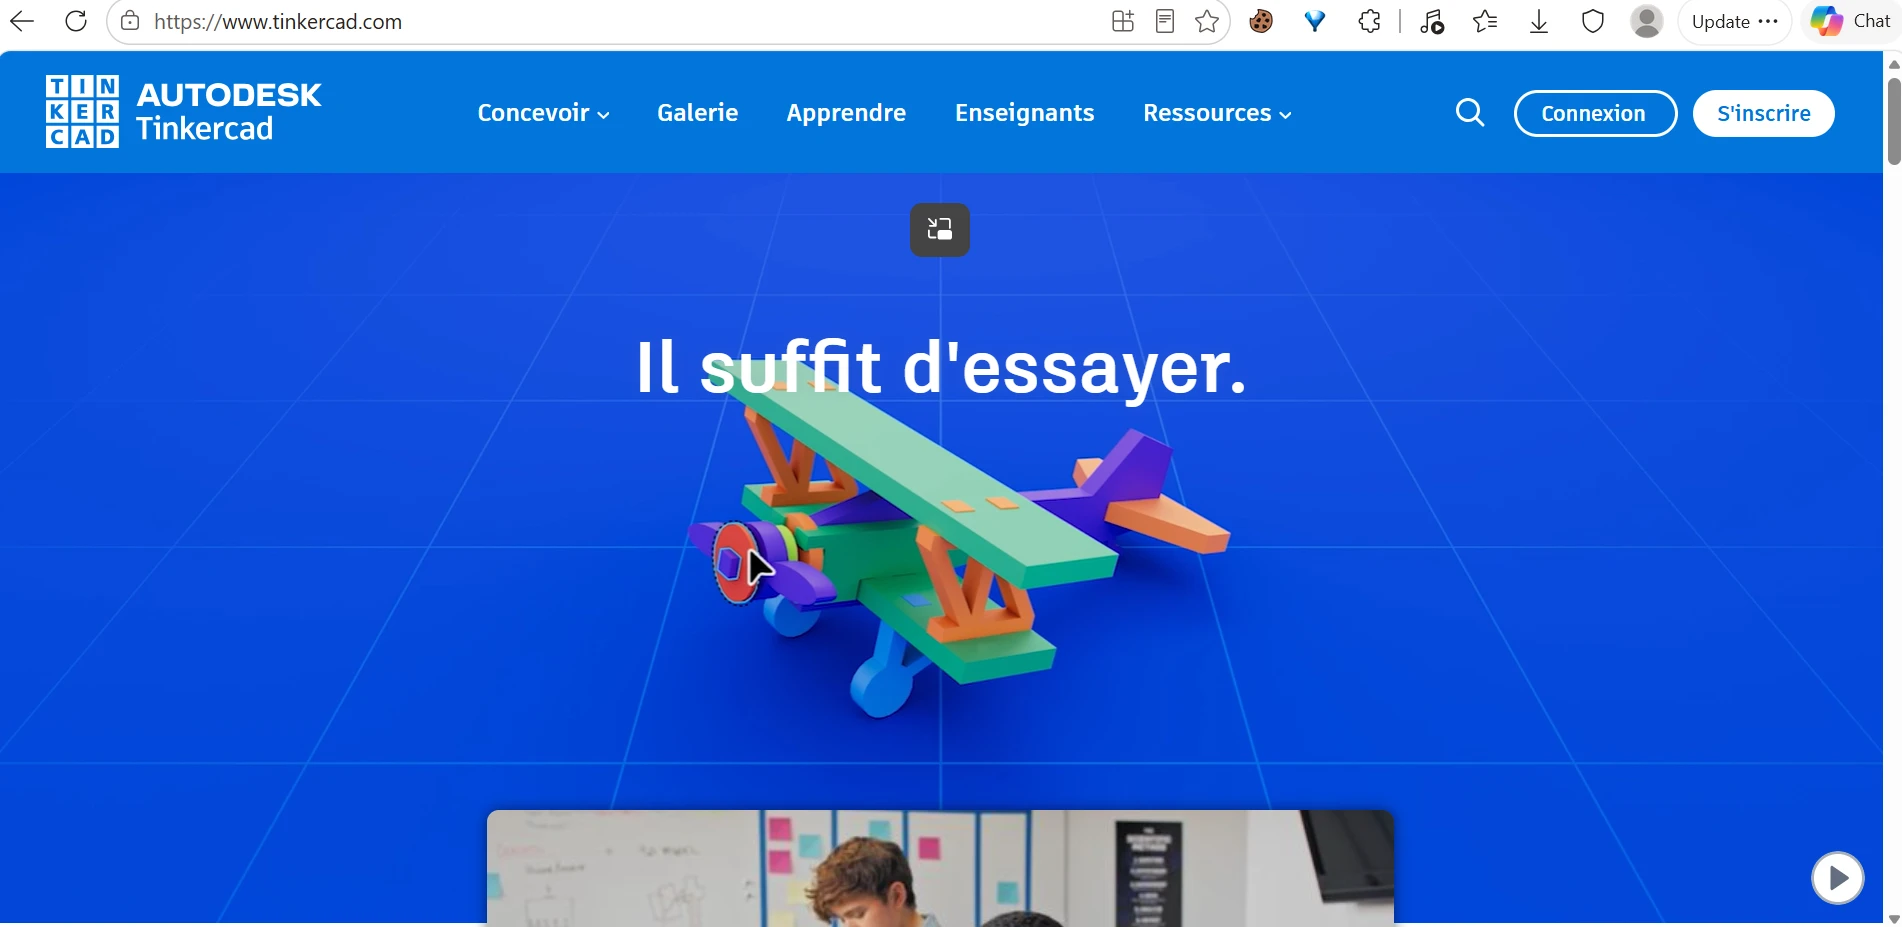
\includegraphics[width=58mm]{assets/T01_site.png}};
\draw[bleufonce!75,line width=.5pt,rounded corners=.8mm]
  ($(current page.north west)+(136.6mm,-28.6mm)$) rectangle ($(current page.north west)+(195.4mm,-57.7mm)$);

% --- Interface -------------------------------------------------------------------
\pos{10mm}{75mm}{188mm}{\subsect{L'interface de Tinkercad Circuits}}
\begin{scope}[shift={($(current page.north west)+(15mm,-84mm)$)},x=1mm,y=-1mm]
  \node[anchor=north west,inner sep=0pt] at (0,0) {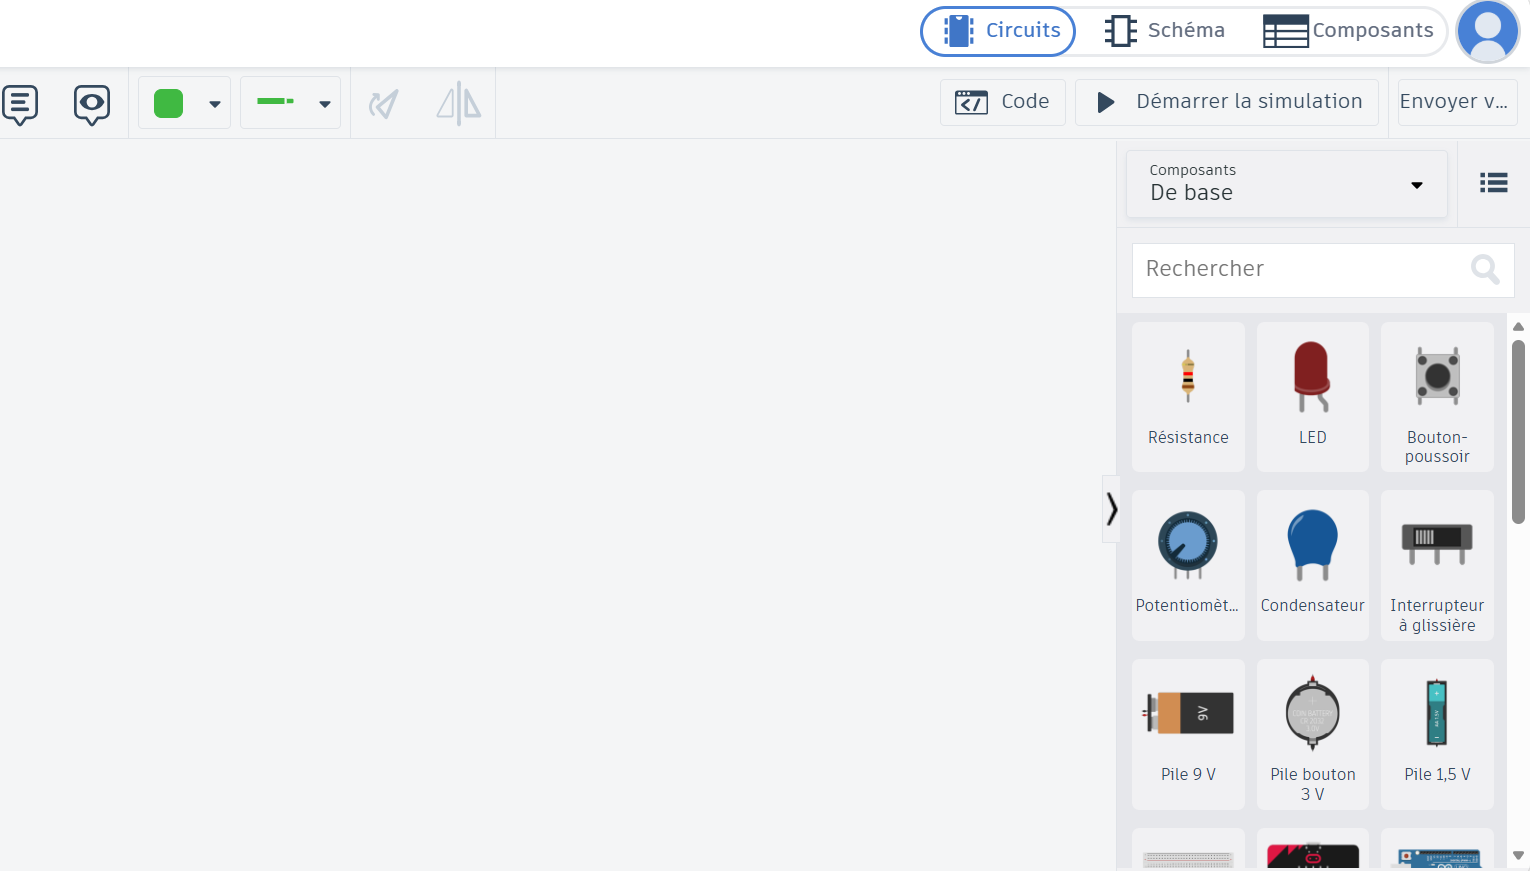
\includegraphics[width=180mm]{assets/T05_interface.png}};
  \draw[bleufonce!75,line width=.55pt,rounded corners=1mm] (-.4,-.4) rectangle (180.4,102.9);
  % 1 px de la capture = 180/1530 mm
  \marque{(105,3.5)}{1}
  \marque{(61.2,12.1)}{2}
  \marque{(118,16.8)}{3}
  \marque{(144,16.8)}{4}
  \marque{(131.4,38.8)}{5}
  \marque{(64.7,56.5)}{6}
\end{scope}
\pos{15mm}{190mm}{182mm}{{\color{bleugris}\fontsize{8.5}{10.3}\selectfont Figure 5 --- Interface de Tinkercad Circuits à l'ouverture d'un nouveau circuit : les six repères désignent les zones à connaître.}}

% --- Légende ----------------------------------------------------------------------
\pos{14mm}{200mm}{86mm}{{\smallfont \textcolor{bleufonce}{\textbf{1. Onglets de vue :}} \textbf{Circuits} (montage), \textbf{Schéma} (schéma électrique) et \textbf{Composants} (liste).}}
\pos{109mm}{200mm}{88mm}{{\smallfont \textcolor{bleufonce}{\textbf{2. Barre d'outils :}} notes, couleur et type de fil, rotation et symétrie.}}
\pos{14mm}{213mm}{86mm}{{\smallfont \textcolor{bleufonce}{\textbf{3. Code :}} programmer l'Arduino en \textbf{blocs} ou en \textbf{texte}.}}
\pos{109mm}{213mm}{88mm}{{\smallfont \textcolor{bleufonce}{\textbf{4. Démarrer la simulation :}} lancer (puis arrêter) la simulation du circuit.}}
\pos{14mm}{226mm}{86mm}{{\smallfont \textcolor{bleufonce}{\textbf{5. Panneau Composants :}} liste \textbf{De base} ou \textbf{Tout}, et barre de recherche.}}
\pos{109mm}{226mm}{88mm}{{\smallfont \textcolor{bleufonce}{\textbf{6. Plan de travail :}} glisser les composants et tracer les fils.}}

% --- À retenir ----------------------------------------------------------------------
\draw[bleufonce,line width=.7pt,rounded corners=2mm]
  ($(current page.north west)+(10mm,-243mm)$) rectangle ($(current page.north west)+(200mm,-259mm)$);
\pos{15mm}{245.5mm}{180mm}{{\fontsize{9.4}{11.4}\selectfont \textcolor{bleufonce}{\bfseries À retenir :} Tinkercad s'utilise en ligne et enregistre automatiquement les projets dans le compte de l'utilisateur. La page suivante montre comment créer un circuit.}}

% --- Pied de page -------------------------------------------------------------------
\draw[bleufonce!55,line width=.45pt] ($(current page.south west)+(10mm,14.7mm)$) --
  ($(current page.south east)+(-10mm,14.7mm)$);
\node[anchor=south west,inner sep=0pt,text=bleufonce!80] at ($(current page.south west)+(10mm,7.4mm)$)
  {\fontsize{9.5}{11}\selectfont 2026/2027};
\node[anchor=south east,inner sep=0pt,text=bleufonce!80] at ($(current page.south east)+(-10mm,7.4mm)$)
  {\fontsize{9.5}{11}\selectfont Page 6};
\end{tikzpicture}
\null
\end{document}
